\documentclass[12pt,letterpaper]{article}
\usepackage{preamble}
\usepackage{graphicx}
\usepackage{subcaption}

%%%%%%%%%%%%%%%%%%%%%%%%%%%%%%%%%%%%%%%%%%
%%%% Edit These for yourself
%%%%%%%%%%%%%%%%%%%%%%%%%%%%%%%%%%%%%%%%%%
\newcommand\course{}
\newcommand\hwnumber{1}
\newcommand\userID{Marina E. Almenzar}

\begin{document}
\section*{Homework 1}

\subsubsection*{Generate a dataset of two-dimensional points, and choose a random line in the plane as your target function f , where one side of the line maps to $+1$ and the other side to $−$. Let the inputs $x_n\in \mathbb{R}^2$ be random points in the plane, and evaluate the target function $f$ on each $x_n$ to get the corresponding output $y_n = f(x_n)$.
Experiment with the perceptron algorithm in the following settings:}
\begin{enumerate}[leftmargin=!,labelindent=5pt]
    \item Generate a dataset of size $20$. Plot the examples ${(x_n, y_n)}$ as well as the target function $f$ on a plane.
        \begin{figure}[H]
            \centering
            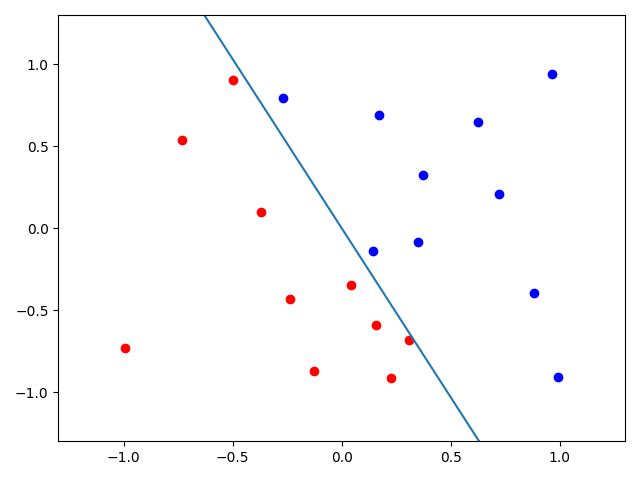
\includegraphics[width=15cm]{images/firstplot.png}
            \caption{}
            \label{fig:1}
        \end{figure}
    \newpage
    \item Run the perceptron algorithm on the dataset. Report the number of updates that the algorithm takes before converging. Plot the examples ${(x_n, y_n)}$, the target function $f$, and the final hypothesis $g$ in the same figure.
        \begin{figure}[H]
        \begin{subfigure}{0.3\textwidth}
        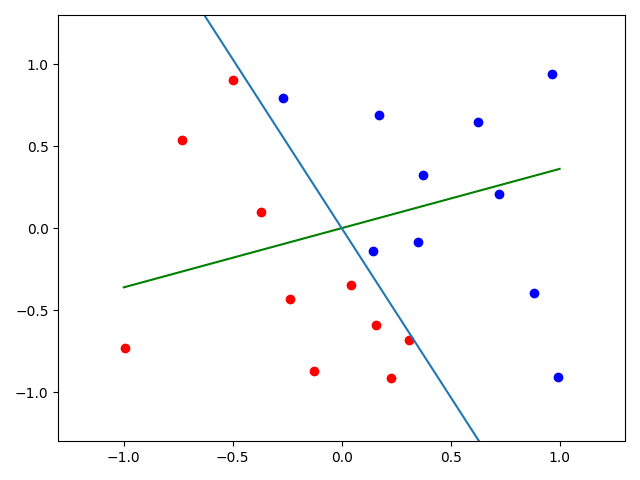
\includegraphics[width=5cm]{images/myplot1.png} 
        \caption{Update 1}
        \label{fig:subim1}
        \end{subfigure}
        \begin{subfigure}{0.3\textwidth}
        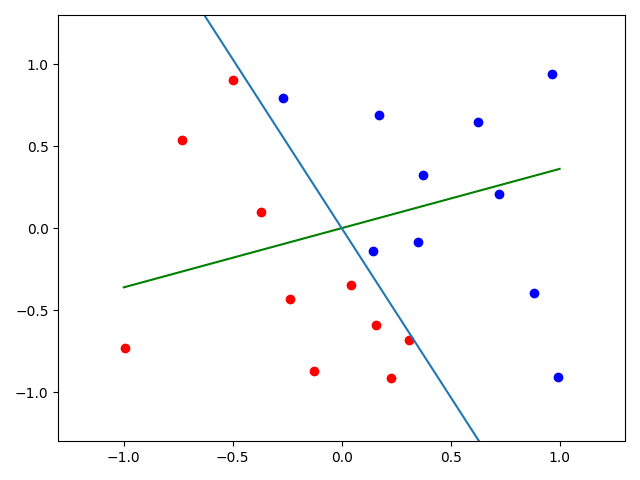
\includegraphics[width=5cm]{images/myplot2.png}
        \caption{Update 2}
        \label{fig:subim2}
        \end{subfigure}
        \begin{subfigure}{0.3\textwidth}
        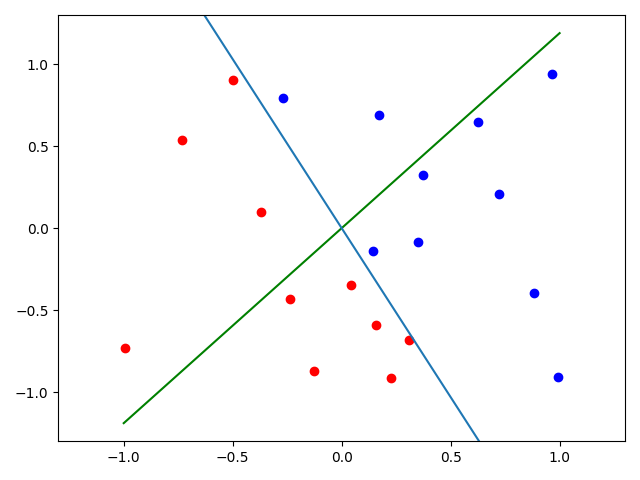
\includegraphics[width=5cm]{images/myplot3.png}
        \caption{Update 3}
        \label{fig:subim2}
        \end{subfigure}
         
        \caption{Updates}
        \label{fig:image2}
        \end{figure}
        \begin{figure}[H]
            \centering
            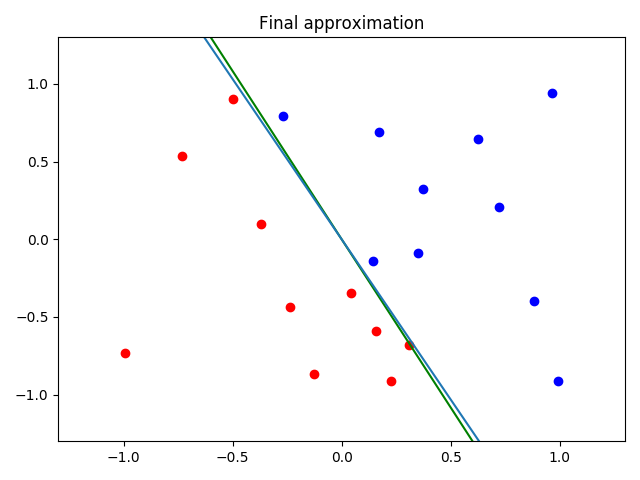
\includegraphics[width=15cm]{images/gplot.png}
            \caption{}
            \label{fig:2}
        \end{figure}
        
    \newpage
    \item Repeat everything in 2. with another randomly generated dataset of size $20$, and compare the result to 2.
        
        \begin{figure}[H]
            \centering
            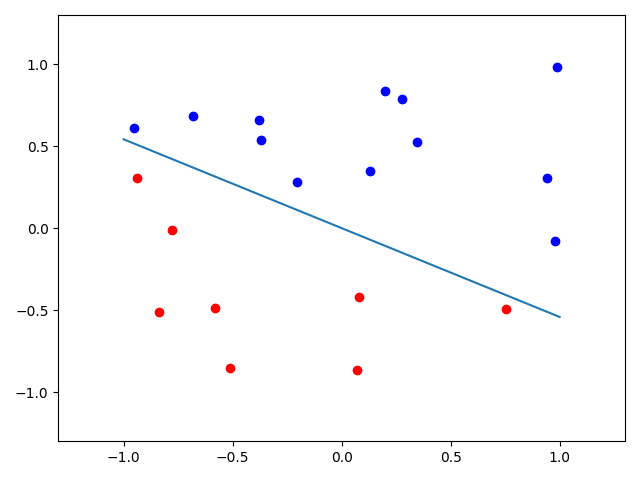
\includegraphics[width=15cm]{images/bfirst.png}
            \caption{Another randomly generated dataset and the target function}
            \label{fig:3}
        \end{figure}

        \begin{figure}[H]
        \begin{subfigure}{0.3\textwidth}
        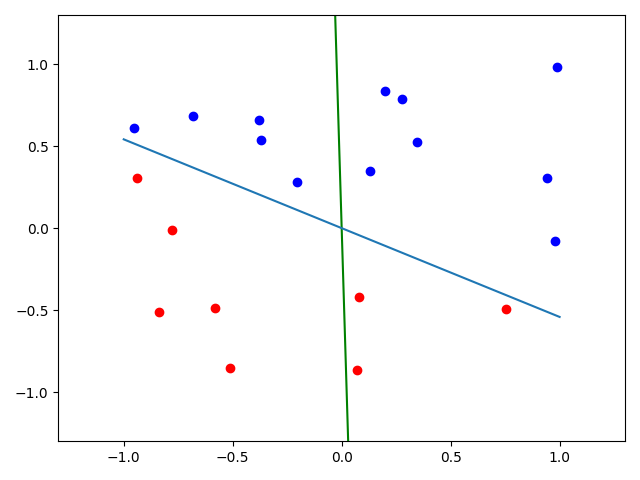
\includegraphics[width=5cm]{images/b3.png} 
        \caption{Update 1}
        \label{fig:subim4}
        \end{subfigure}
        \begin{subfigure}{0.3\textwidth}
        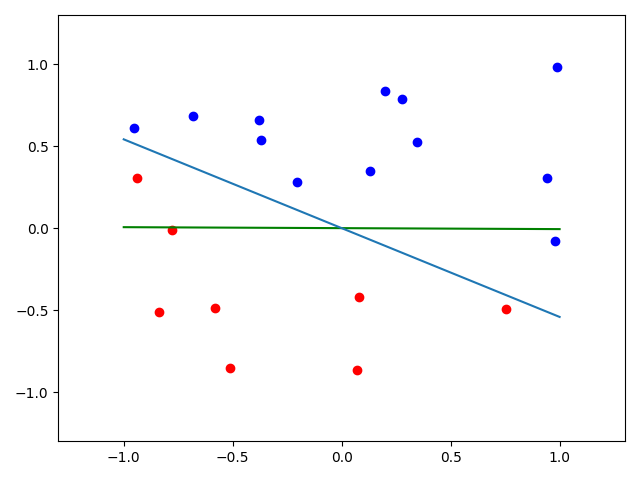
\includegraphics[width=5cm]{images/b4.png}
        \caption{Update 2}
        \label{fig:subim5}
        \end{subfigure}
        \begin{subfigure}{0.3\textwidth}
        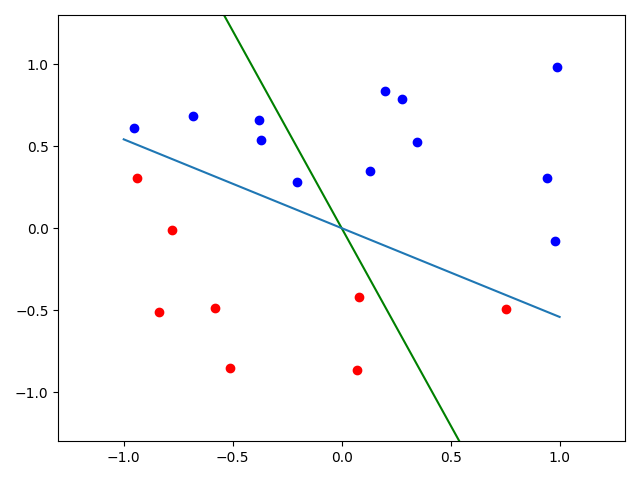
\includegraphics[width=5cm]{images/b5.png}
        \caption{Update 3}
        \label{fig:subim6}
        \end{subfigure}
        
        \begin{subfigure}{0.3\textwidth}
        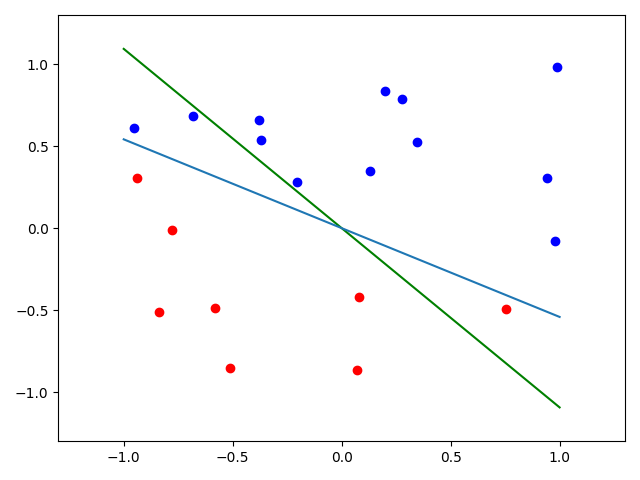
\includegraphics[width=5cm]{images/b6.png} 
        \caption{Update 4}
        \label{fig:subim4}
        \end{subfigure}
        \begin{subfigure}{0.3\textwidth}
        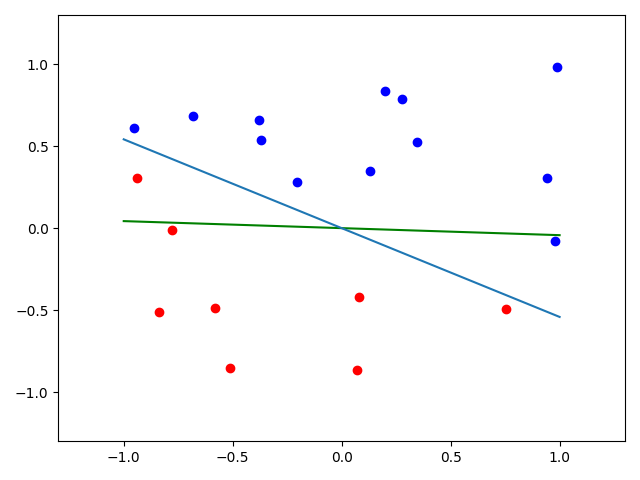
\includegraphics[width=5cm]{images/b7.png}
        \caption{Update 5}
        \label{fig:subim5}
        \end{subfigure}
        \begin{subfigure}{0.3\textwidth}
        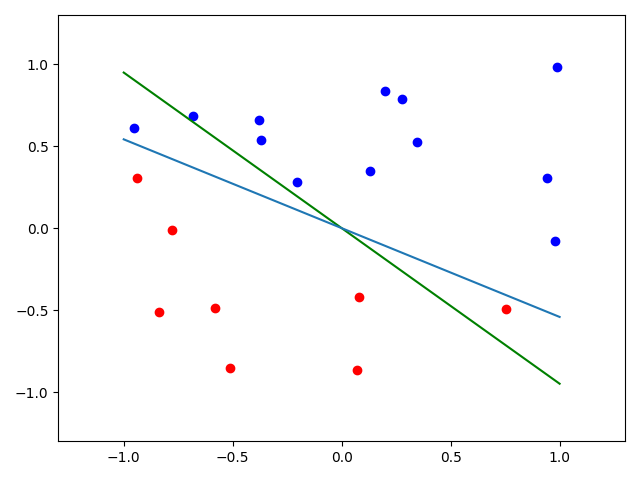
\includegraphics[width=5cm]{images/b8.png}
        \caption{Update 6}
        \label{fig:subim6}
        \end{subfigure}
        
        \begin{subfigure}{0.3\textwidth}
        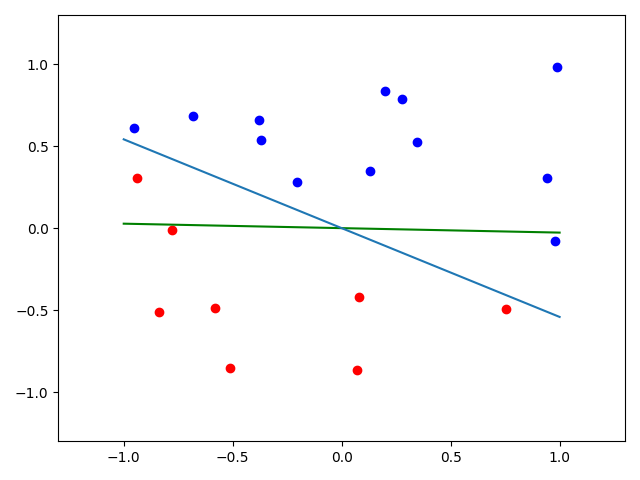
\includegraphics[width=5cm]{images/b9.png} 
        \caption{Update 7}
        \label{fig:subim4}
        \end{subfigure}
        \begin{subfigure}{0.3\textwidth}
        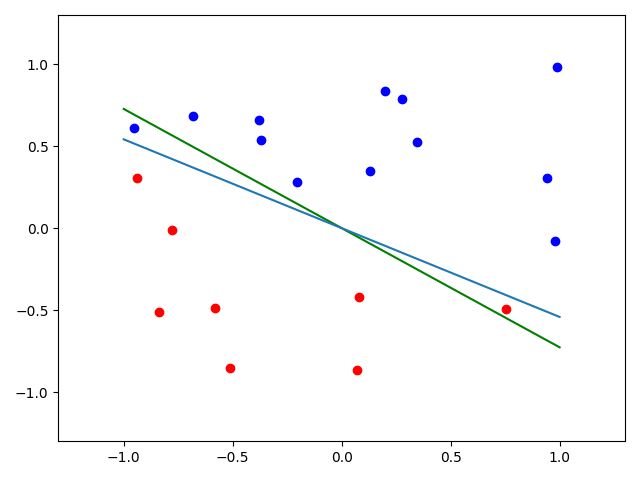
\includegraphics[width=5cm]{images/b10.png}
        \caption{Update 8}
        \label{fig:subim5}
        \end{subfigure}
        \begin{subfigure}{0.3\textwidth}
        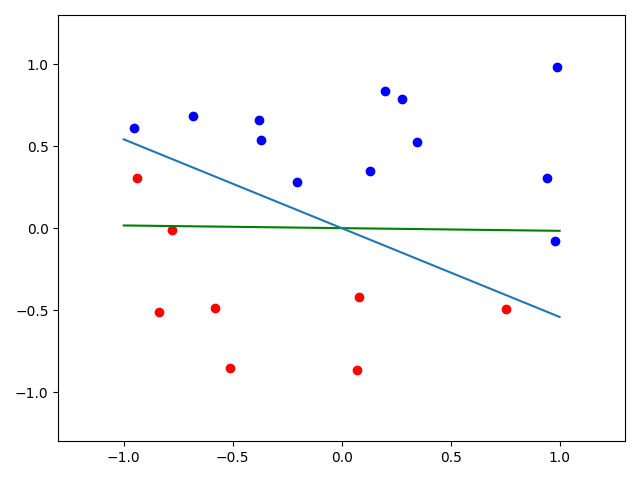
\includegraphics[width=5cm]{images/b11.png}
        \caption{Update 9}
        \label{fig:subim6}
        \end{subfigure}
        \end{figure}
        
        \begin{figure}[H]
            \centering
            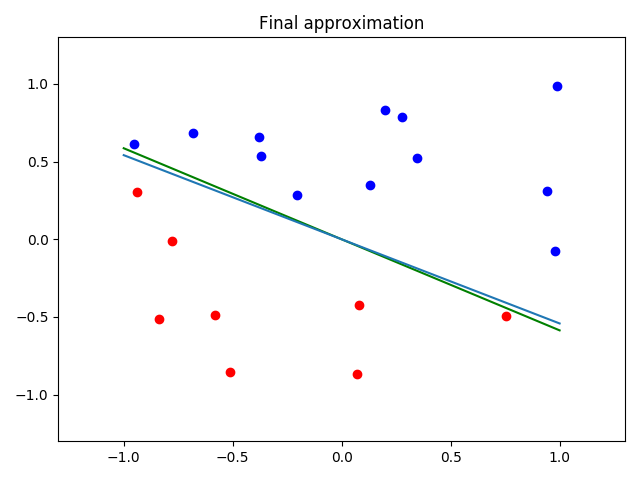
\includegraphics[width=15cm]{images/bfinal.png}
            \caption{}
            \label{fig:3}
        \end{figure}
    \newpage
    \item Repeat everything in 2. with another randomly generated dataset of size $100$, and compare the result to 2.
    
        \begin{figure}[H]
            \centering
            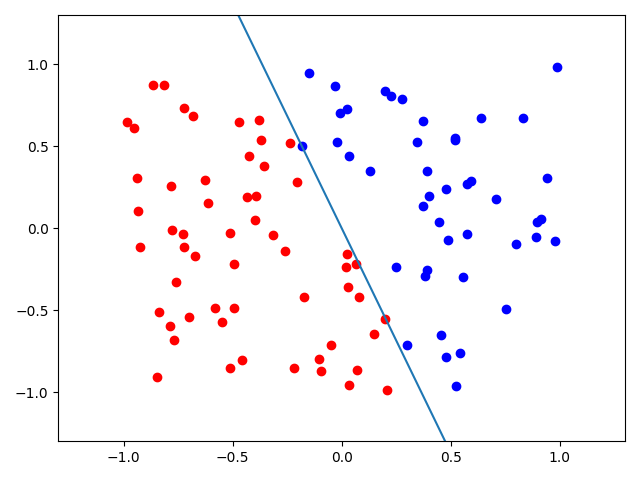
\includegraphics[width=15cm]{images/cfirst.png}
            \caption{Randomly generated dataset of size $100$ and the target function}
            \label{fig:3}
        \end{figure}

        \begin{figure}[H]
        \begin{subfigure}{0.3\textwidth}
        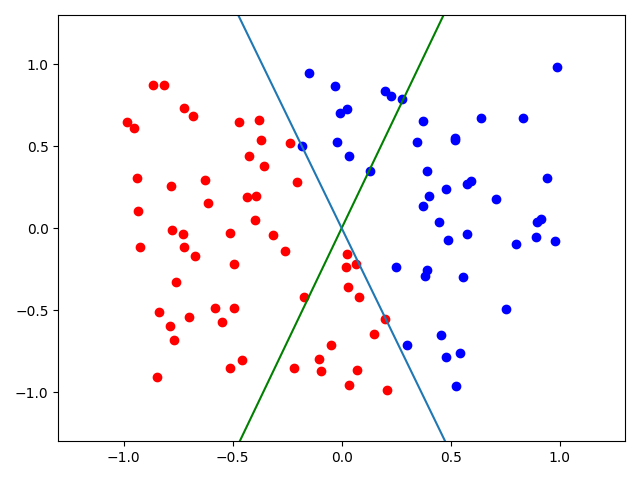
\includegraphics[width=5cm]{images/c1.png} 
        \caption{Update 1}
        \label{fig:subim4}
        \end{subfigure}
        \begin{subfigure}{0.3\textwidth}
        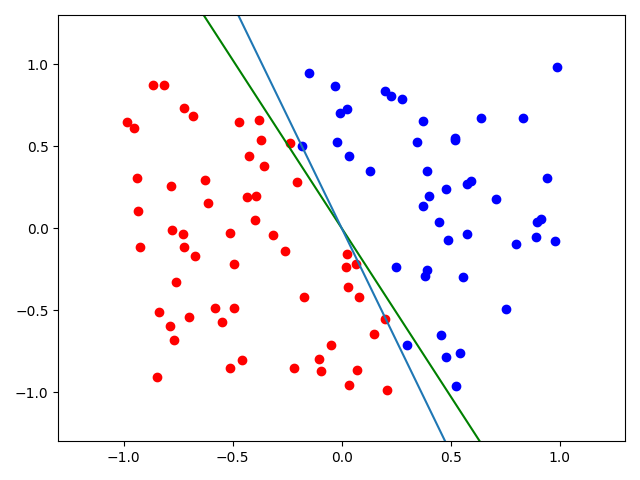
\includegraphics[width=5cm]{images/c2.png}
        \caption{Update 2}
        \label{fig:subim5}
        \end{subfigure}
        \begin{subfigure}{0.3\textwidth}
        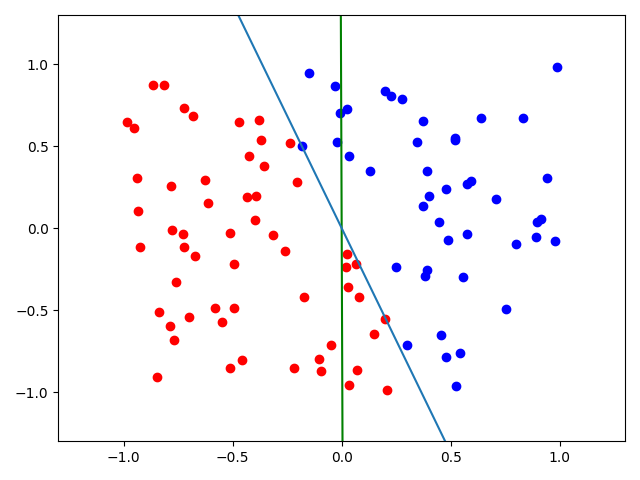
\includegraphics[width=5cm]{images/c3.png}
        \caption{Update 3}
        \label{fig:subim6}
        \end{subfigure}
        \end{figure}
        
        \begin{figure}[H]
            \centering
            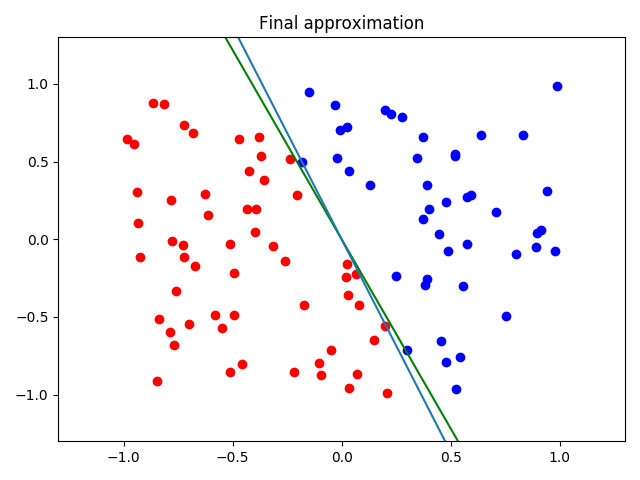
\includegraphics[width=15cm]{images/cfinal.png}
            \caption{}
            \label{fig:3}
        \end{figure}
    \newpage
    \item Repeat everything in 2. with another randomly generated dataset of size $1000$, and compare the result to 2.
    
        \begin{figure}[H]
            \centering
            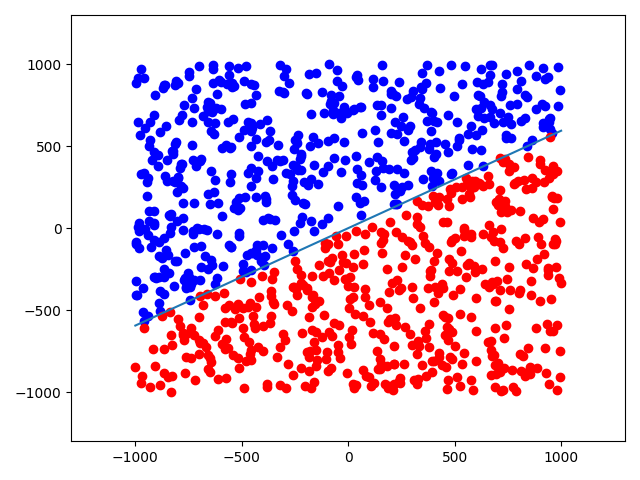
\includegraphics[width=15cm]{images/dfirst.png}
            \caption{Randomly generated dataset of size $1000$ and the target function}
            \label{fig:3}
        \end{figure}
        
        \begin{figure}[H]
            \centering
            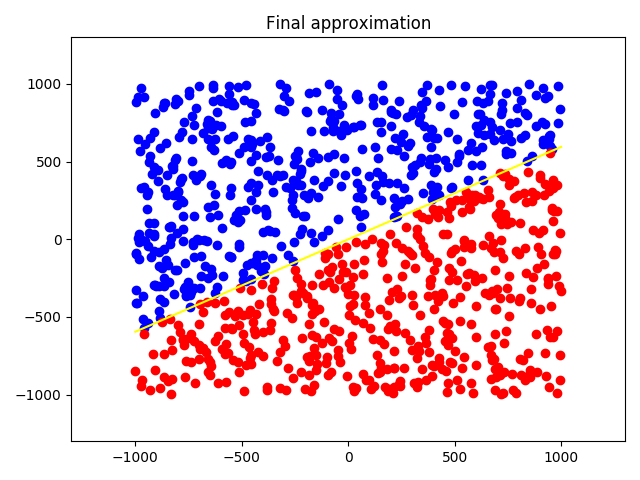
\includegraphics[width=15cm]{images/dfinal.png}
            \caption{Final hypothesis (in yellow) $g$ after \textbf{97 iterations}}
            \label{fig:3}
        \end{figure}
    \item Modify the experiment such that $x_n\in \mathbb{R}^{10}$ instead of $\mathbb{R}^2$. Run the algorithm on a randomly generated dataset of size $1000$. How many updates does the algorithm take to converge?
    
    \textbf{The algorithm takes 3512 updates to converge.}
    \newpage
    \item Summarize your conclusions regarding the accuracy and running time of the algorithm as a function of $N$ (the number of data points) and d (the number of dimensions).

        \subitem $\mathbb{R}^{2}$, dataset of size $20$ (10 updates): \textbf{0.0005986690521240234 seconds}
        \subitem $\mathbb{R}^{2}$, dataset of size $100$ (4 updates): \textbf{0.0011091232299804688 seconds}
        \subitem $\mathbb{R}^{2}$, dataset of size $1000$ (97 updates): \textbf{0.03201484680175781 seconds}
        \subitem $\mathbb{R}^{10}$, dataset of size $1000$ (3512 updates): \textbf{1.349951982498169 seconds}
        
        \subsubsection*{Conclusions}
        \subitem A larger quantity of samples does not imply a greater number of updates (see cases first and two) but (obviously) it does affect the execution time.
        \subitem This measures depend on the dispersion of the samples, which is not proportional to the number of samples in each example. This disadvantages the cases with a high number of samples.

    
        
\end{enumerate}
\end{document}
